\begin{figure}[h!]
    \centering
    \caption{Effects of \emph{Plan Cuadrante} on Perceived Police Performance and Police Presence}
    \label{fig:figure4}
    \begin{subfigure}{0.495\textwidth}
        \centering
        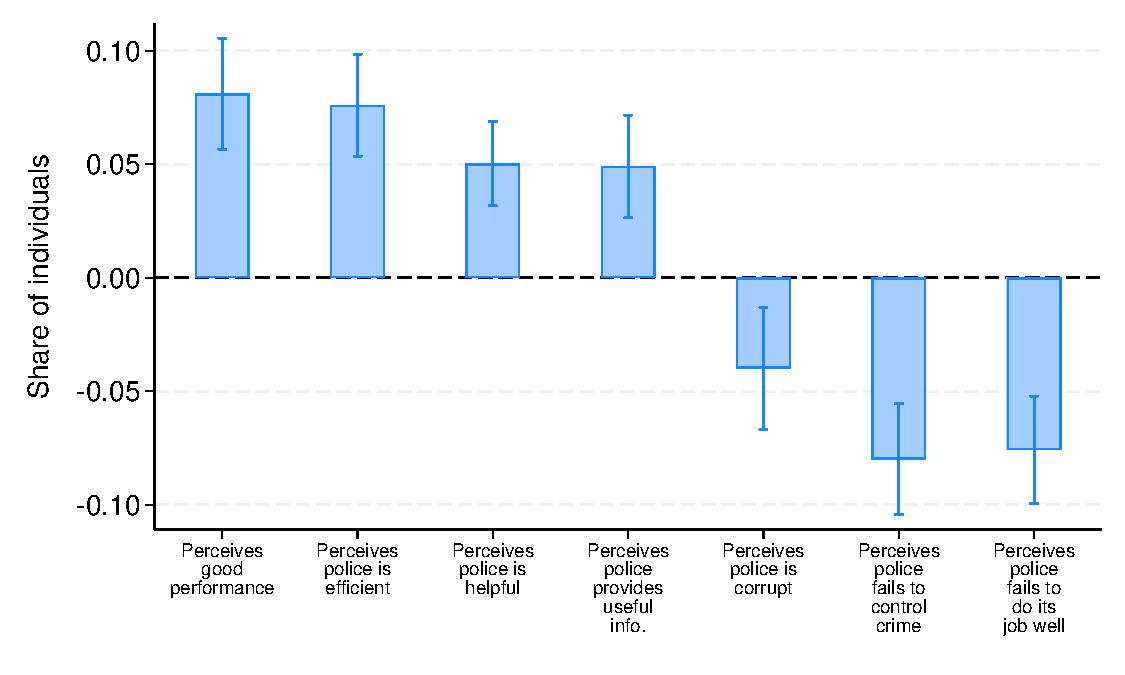
\includegraphics[width=\textwidth]{../manuscript/Graphs/combined_PCttest_2.pdf}
        \caption{Effects on perceived police performance measures}
    \end{subfigure}%
    ~ 
    \begin{subfigure}{0.495\textwidth}
        \centering
        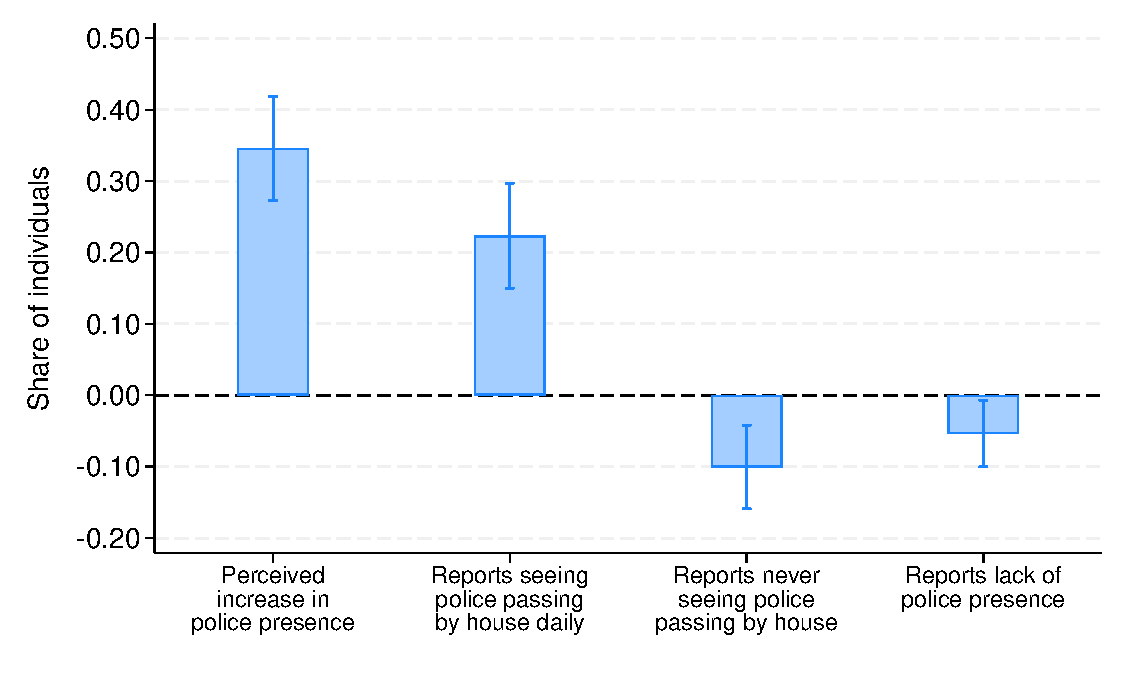
\includegraphics[width=\textwidth]{../manuscript/Graphs/results_policepresence.pdf}
        \caption{Effects on police sighting frequency}
    \end{subfigure}%
    \\[12pt]
    \begin{minipage}{0.99\textwidth}
    Notes: Panel (a) reports the association between \emph{Plan Cuadrante} and different measures of subjective police performance available in ENUSC round 2005. These are the share of individuals that believe Carabineros perform well, are helpful, are corrupt, are efficient, failed to control crime, failed to do their job well, and are well informed. We compare these measures in municipalities in the main analytical sample where \emph{Plan Cuadrante} was already implemented before 2006 and in municipalities where the program was implemented after 2005. This panel includes 8,495, 7,975, 8,326, 7,439, 6,621, 7,712, 7,889 observations, respectively, corresponding to each bar from left to right. The graphs display the estimated coefficients and 95\% confidence intervals. Standard errors are clustered at the municipality level. Panel (b) reports the effects of \emph{Plan Cuadrante} on different measures of police presence: the probability of perceiving an increase in police presence, seeing police pass by their house daily, never see police pass by their house, and complains about lack of police surveillance. Information on the three first measures is only available for ENUSC rounds 2003, 2005 and 2006, while information on complaints about the lack of police surveillance is available for ENUSC rounds 2003-2012. This panel includes 22,971, 15,151, 15,151, and 120,033 observations, respectively, corresponding to each bar from left to right. The estimation is conducted using the difference-in-differences estimator for staggered treatment adoption developed in \citet{Callaway}. The graphs display the estimated coefficients and 95\% confidence intervals. Standard errors are clustered at the municipality level using the wild bootstrapping procedure. 
    \end{minipage}
\end{figure}

